\documentclass{standalone}

\usepackage{tikz}
\usetikzlibrary{calc}
\usetikzlibrary{patterns}

\usepackage[T2A]{fontenc}

\newlength{\len}
\setlength{\len}{.3mm}

\begin{document}

\begin{tikzpicture}[x=\len, y=\len]

  \path (0, 0) node(a){
    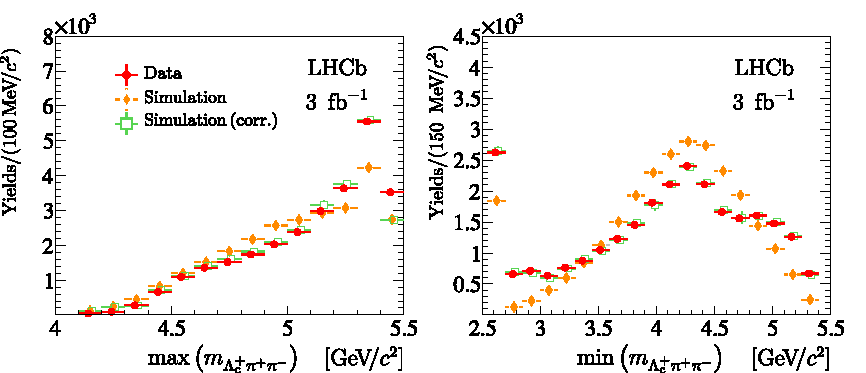
\includegraphics[width=200\len]{reweighting-lcpipi}
  };
  \path (a.south) node[anchor=north](b){
    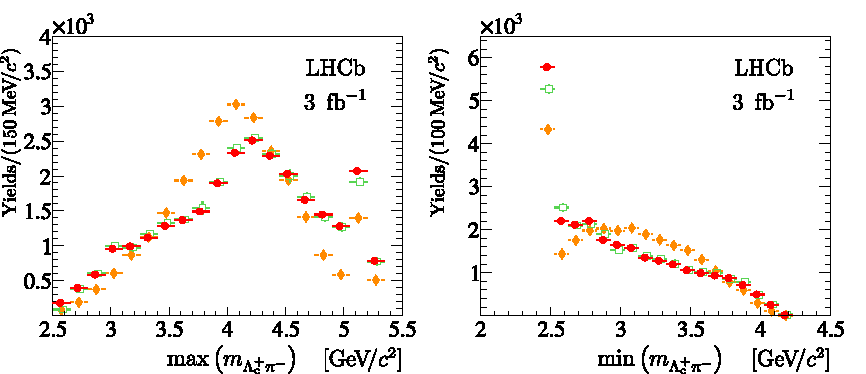
\includegraphics[width=200\len]{reweighting-lcpim}
  };
  \path (a.south east) node[anchor=west](c){
    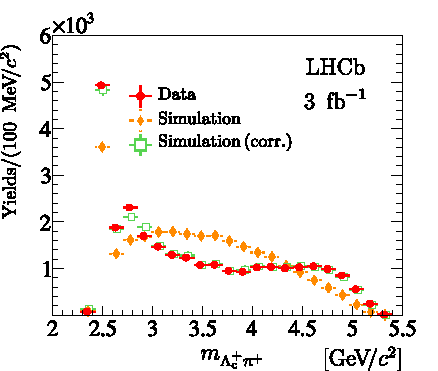
\includegraphics[width=100\len]{reweighting-lcpip}
  };

  \path (a.center) ++(20, -5) coordinate(ar);
  \path (b.center) ++(30, 5) coordinate(br);
  \path (c.west) ++(30, 0) coordinate(cr);

  \draw[thick, line width=1\len, red] (ar) ellipse (15 and 30);
  \draw[thick, line width=1\len, red] (br) ellipse (17 and 30);
  \draw[thick, line width=1\len, red] (cr) ellipse (17 and 30);

  \path (a.north east) ++(50, -20) node(text){Резонансы};
  \draw[->] (text.south west) to[out=210, in=10] ($(ar) +(17, 0)$);
  \draw[->] ($(text.south west)+(9, 0)$) to[out=250, in=40] ($(br) +(20, 8)$);
  \draw[->] ($(text.south)+(15, 0)$) to[out=270, in=40] ($(cr) +(20, 20)$);
  % \draw[->] plot[smooth] coordinates{
  %   (text.south west) ($.5*(ar) + .5*(text.south west) + (15, -3)$) ($(ar) +(17, 0)$)
  % };
  % \draw[->] plot[smooth] coordinates{
  %   ($(text.south west)+(5, 0)$) ($.5*(br) + .5*(text.south west) + (15, -3)$) ($(br) +(20, 8)$)
  % };
  % \draw[->] plot[smooth] coordinates{
  %   ($(text.south)+(15, 0)$) ($.5*(cr) + .5*(text.south) + (20, 10)$) ($(cr) +(20, 20)$)
  % };

\end{tikzpicture}

\end{document}
